% case name
\chapter{refinement}
%
%
% - Purpose & Description:
%     These first two parts give reader short details about the test case,
%     the physical phenomena involved, the geometry and specify how the numerical solution will be validated
\section{Purpose}
This example illustrates the manipualtions that can be done within a Serafin
file.
%
\section{Description}
The computation refine the mesh by splitting each triangle into 4.

%
% - Physical parameters:
%     This part specifies details all the physical parameters
%\subsection{Physical parameters}
%
% Experimental results (if needed)
%\subsection{Experimental results}
%
% bibliography can be here or at the end
%\subsection{Reference}
%
% Section for computational options
%\section{Computational options}
%
% - Mesh:
%     This part describes the mesh used in the computation
%\subsection{Mesh}
%
% - Initial and boundary conditions:
%     This part details both initial and boundary conditions used to simulate the case
%\subsection{Initial and boundary conditions}
%
% - Numerical parameters:
%     This part is used to specify the numerical parameters used
%     (adaptive time step, mass-lumping when necessary...)
%\subsection{Numerical parameters}
%
% - Results:
%     We comment in this part the numerical results against the reference ones,
%     giving understanding keys and making assumptions when necessary.
\section{Results}
The figure \ref{fig:refinement:inimesh} shows the initial mesh
and the figure \ref{fig:refinement:newmesh} shows the newly refined mesh:
\begin{figure}[H]%
\begin{center}
%
  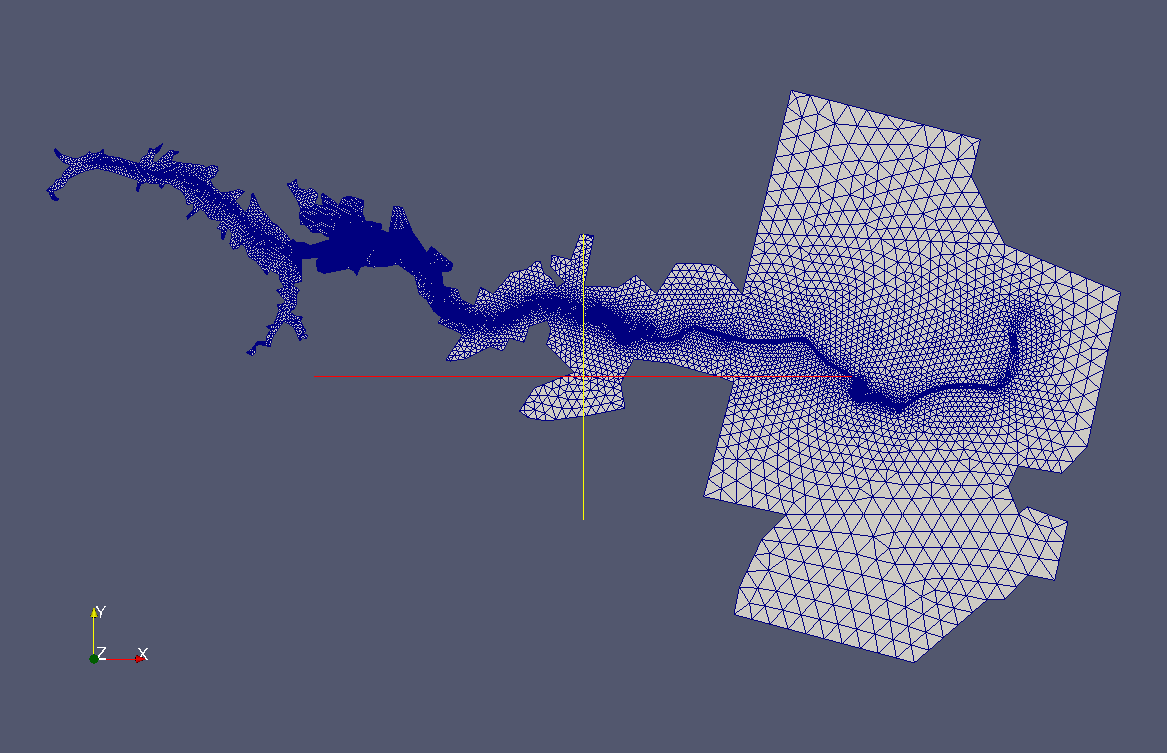
\includegraphics[width=0.9\textwidth]{inimesh}
%
\end{center}
\caption
{The initial mesh}
\label{fig:refinement:inimesh}
\end{figure}
%
\begin{figure}[H]%
\begin{center}
%
  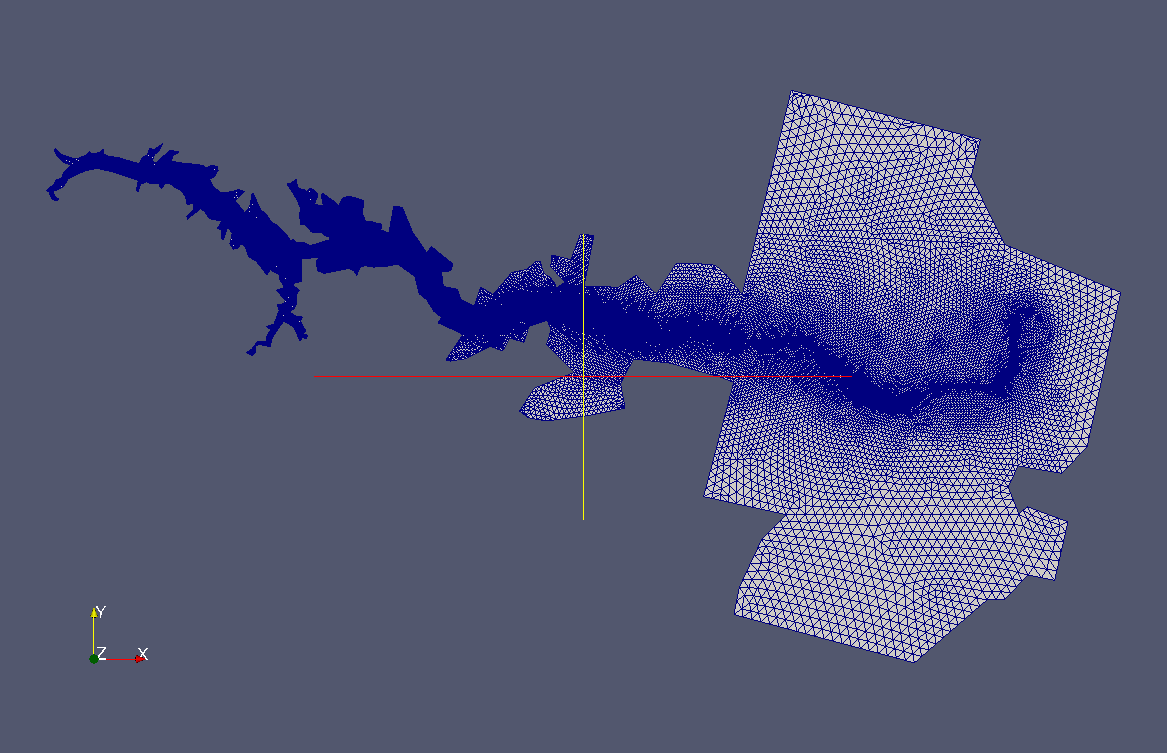
\includegraphics[width=0.9\textwidth]{newmesh}
%
\end{center}
\caption
{The refined mesh}
\label{fig:refinement:newmesh}
\end{figure}
%
% bibliography
%\section{Reference}
